\documentclass{beamer}
\usepackage[utf8]{inputenc}
\usepackage[T1]{fontenc}
\setbeamertemplate{caption}[numbered]

% \title{\textbf{SlimGuard: A Secure and Memory-Efficient Heap Allocator}}
\title{\textbf{SlimGuard: A Secure and  Memory Efficient Heap Allocator}}
\date{12/11/2019}
\author{\underline{Beichen Liu},  Pierre Olivier,  Binoy Ravindran\\
\small ECE, Virginia Tech}

\graphicspath{{./include/}}

\usetheme{ssrg}

\begin{document}

%% Page 1
\begin{frame}
\titlepage
\end{frame}

%% Page 2
\section{Background and Motivation}
\subsection{Motivation}
\begin{frame}
		\frametitle{\secname}
    \framesubtitle{\subsecname}
    \begin{figure}
      \centering
      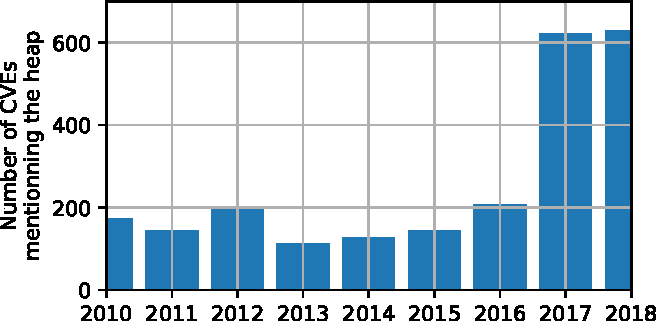
\includegraphics{CVE.pdf}
      \\Number of heap-related CVE entries since 2010.

    \end{figure}
\end{frame}


% Page 3
\section{Background and Motivation}
\subsection{Heap Vulnerabilities}
\begin{frame}
		\frametitle{\secname}
    \framesubtitle{\subsecname}
    \begin{itemize}
      \item buffer overflow, buffer overread
          \begin{figure}
              \centering
              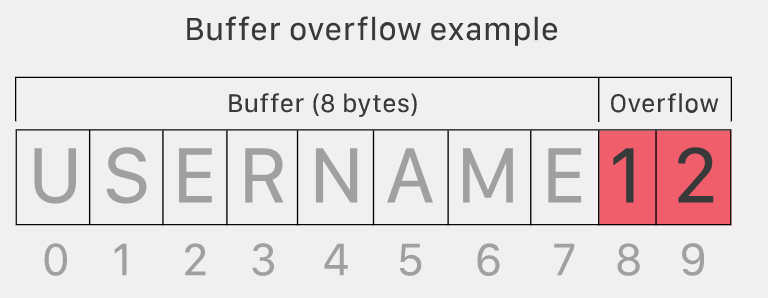
\includegraphics[scale=0.3]{buffer_overflow}
              \\Buffer overflow example
          \end{figure}
      \item use-after-free/double free
      \item invalid free
    \end{itemize}
\end{frame}

% Page 4
\section{Background and Motivation}
\subsection{Related Works}
\begin{frame}
  \frametitle{\secname}
  \framesubtitle{\subsecname}

    One solution for these heap vulnerabilities is to use a secure heap
    allocator, aka use a secure malloc algorithm.\\
  \begin{itemize}
    \item OpenBSD
      \begin{itemize}
        \item segragation of metadata
        \item randomized allocation
        \item security guarantees are not competitive
      \end{itemize}
  \item DieHarder(PLDI'06)
      \begin{itemize}
          \item randomized allocation
          \item over-provisioning
          \item memory overhead is large
      \end{itemize}
  \item FreeGuard(CCS'17) and Guarder(USENIX'18)
      \begin{itemize}
        \item high performance
        \item high security guarantee
        \item memory overhead is large
      \end{itemize}
  \end{itemize}
\end{frame}

% Page 5
\section{Background and Motivation}
\subsection{Related Works}
\begin{frame}
  \frametitle{\secname}
  \framesubtitle{\subsecname}

  Existing secure allocator are either not really secure or \textbf{not memory
efficient}.

\end{frame}

% Page 6
\section{Design and Implementation}
\begin{frame}
	\frametitle{\secname}
  \begin{figure}
      \centering
      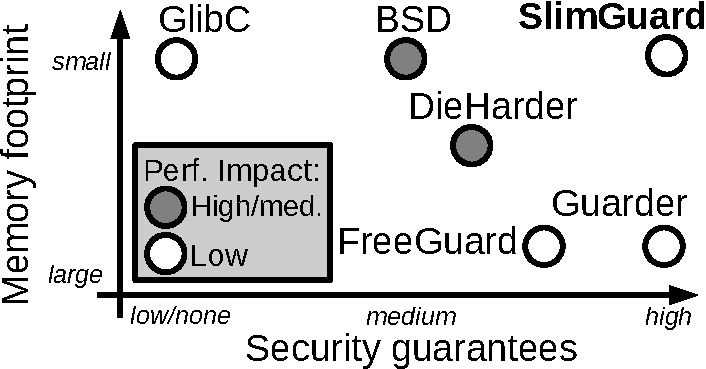
\includegraphics[scale=0.6]{design-space.pdf}
      \\SlimGuard in the secure allocators design space.
  \vspace{-4pt}
  \end{figure}
    Design Objective: \textbf{memory efficiency}, competitive security guarantees,
    and negligible performance overhead.
\end{frame}

% Page 7
\section{Design and Implementation}
\subsection{General Design}
\begin{frame}
	  \frametitle{\secname}
    \framesubtitle{\subsecname}
    \begin{enumerate}
        \item size class management
        \item malloc path
        \item free path
        \item multithreading, binary compatibility
    \end{enumerate}
\end{frame}

% Page 8
\section{Design and Implementation}
\subsection{Size Classes Management}
\begin{frame}
	  \frametitle{\secname}
    \framesubtitle{\subsecname}
    free-list(e.g., ptmallocv2)
    \begin{itemize}
        \item round size up to a multiple of 8 or 16 bytes
        \item store the size right before the heap object
    \end{itemize}
    \begin{figure}
      \centering
      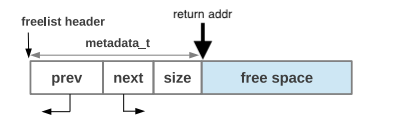
\includegraphics[scale=0.6]{inline_metadata}
      \\ Inline metadata example
    \end{figure}
\end{frame}

% Page 9
\section{Design and Implementation}
\subsection{Size Classes Management}
\begin{frame}
  	\frametitle{\secname}
    \framesubtitle{\subsecname}
    bibop style (e.g., OpenBSD, Guarder)
    \begin{itemize}
        \item power-of-2 class size
        \item a memory region are equally divided into classs size
    \end{itemize}
    \begin{figure}
      \centering
      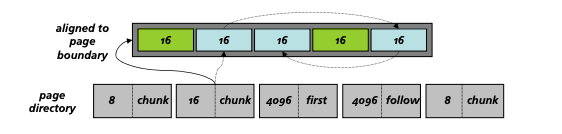
\includegraphics[scale=0.6]{bibop_heap}
      \\ BIBOP heap example
    \end{figure}
\end{frame}

% Page 10
\section{Design and Implementation}
\subsection{SlimGuard Size Classed Management}
\begin{frame}
	\frametitle{\secname}
    \framesubtitle{\subsecname}
    SlimGuard: Fine-grained size class management
    \begin{figure}
      \centering
      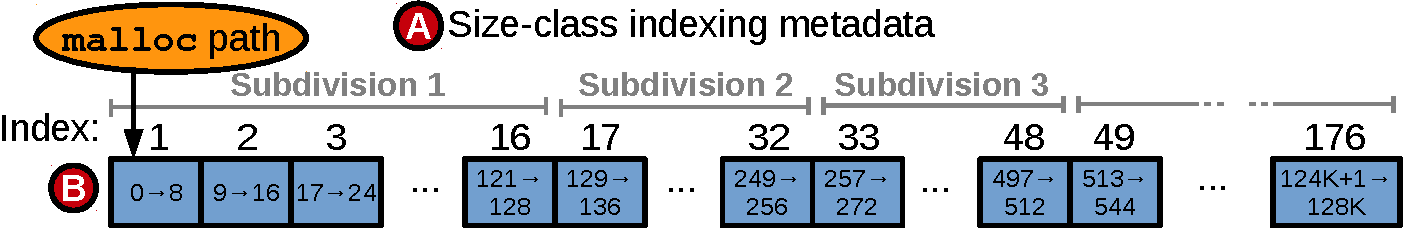
\includegraphics[scale=0.4]{overview1.pdf}
      \\ SlimGuard Design Space
    \end{figure}
\end{frame}

% Page 11
\section{Design and Implementation}
\subsection{SlimGuard Malloc Path}
\begin{frame}[fragile]
		\frametitle{\secname}
    \framesubtitle{\subsecname}
    \begin{verbatim}
    void *pointer = malloc(x);
    \end{verbatim}
    \begin{figure}
      \centering
      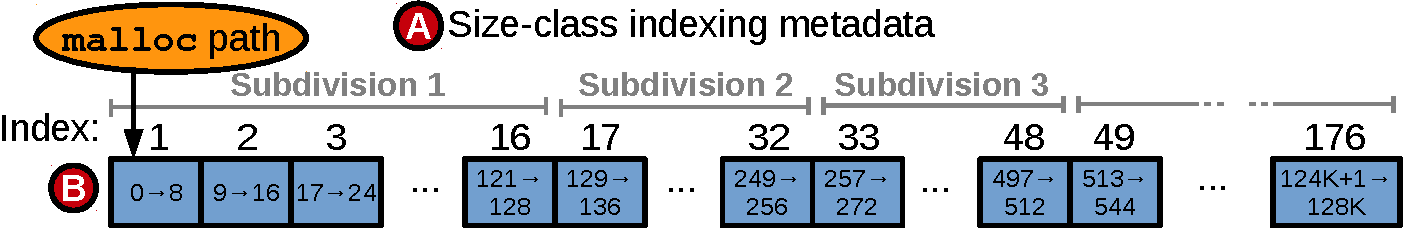
\includegraphics[scale=0.4]{overview1.pdf}
      \\ SlimGuard Design Space
    \end{figure}
\end{frame}

% Page 12
\section{Design and Implementation}
\subsection{SlimGuard Malloc Path}
\begin{frame}[fragile]
		\frametitle{\secname}
    \framesubtitle{\subsecname}
    \begin{verbatim}
    void *pointer = malloc(x);
    \end{verbatim}
    \begin{figure}
      \centering
      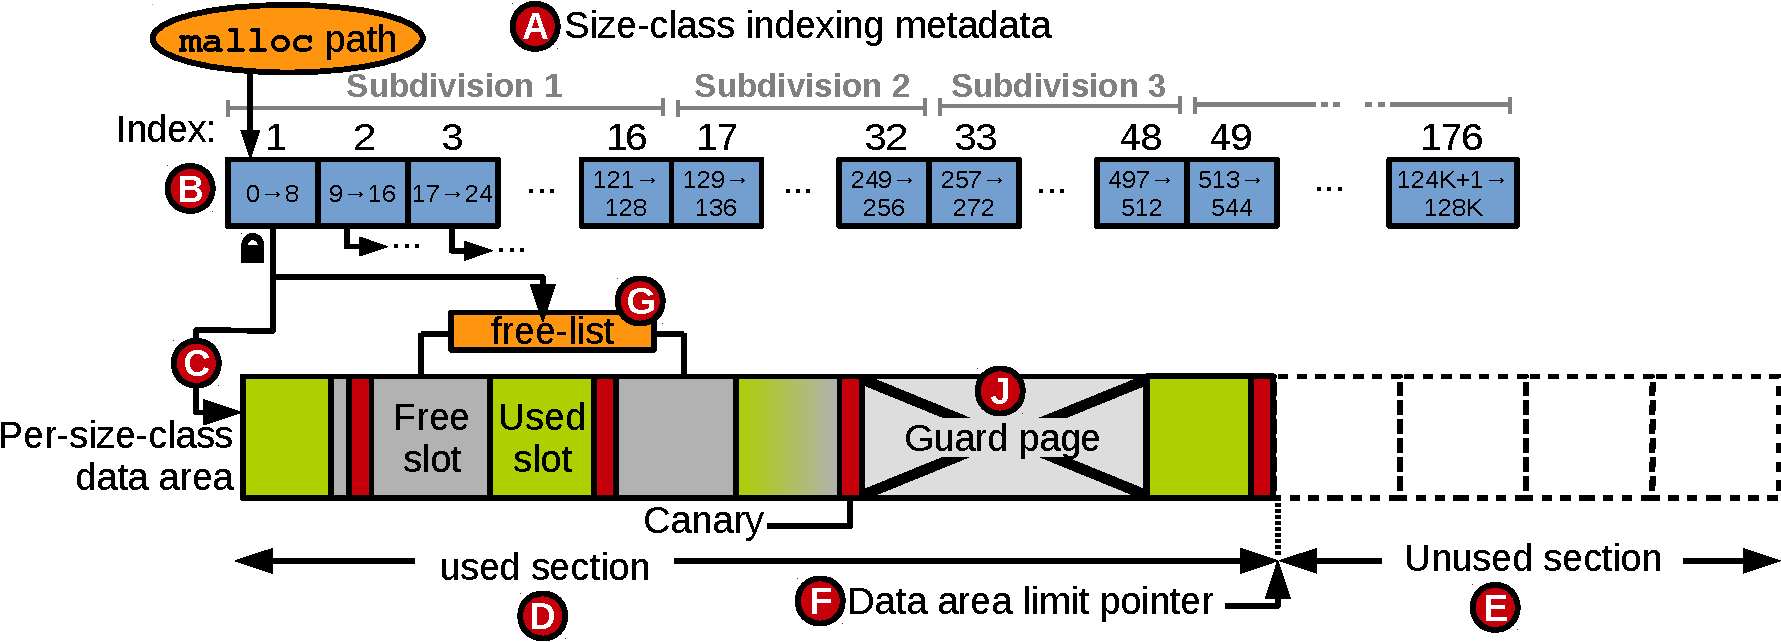
\includegraphics[scale=0.35]{overview2.pdf}
      \\ SlimGuard Design Space
    \end{figure}
\end{frame}

% Page 13
\section{Design and Implementation}
\subsection{SlimGuard Free Path}
\begin{frame}[fragile]
		\frametitle{\secname}
    \framesubtitle{\subsecname}
    \begin{verbatim}
    free(pointer);
    \end{verbatim}
    \begin{figure}
      \centering
      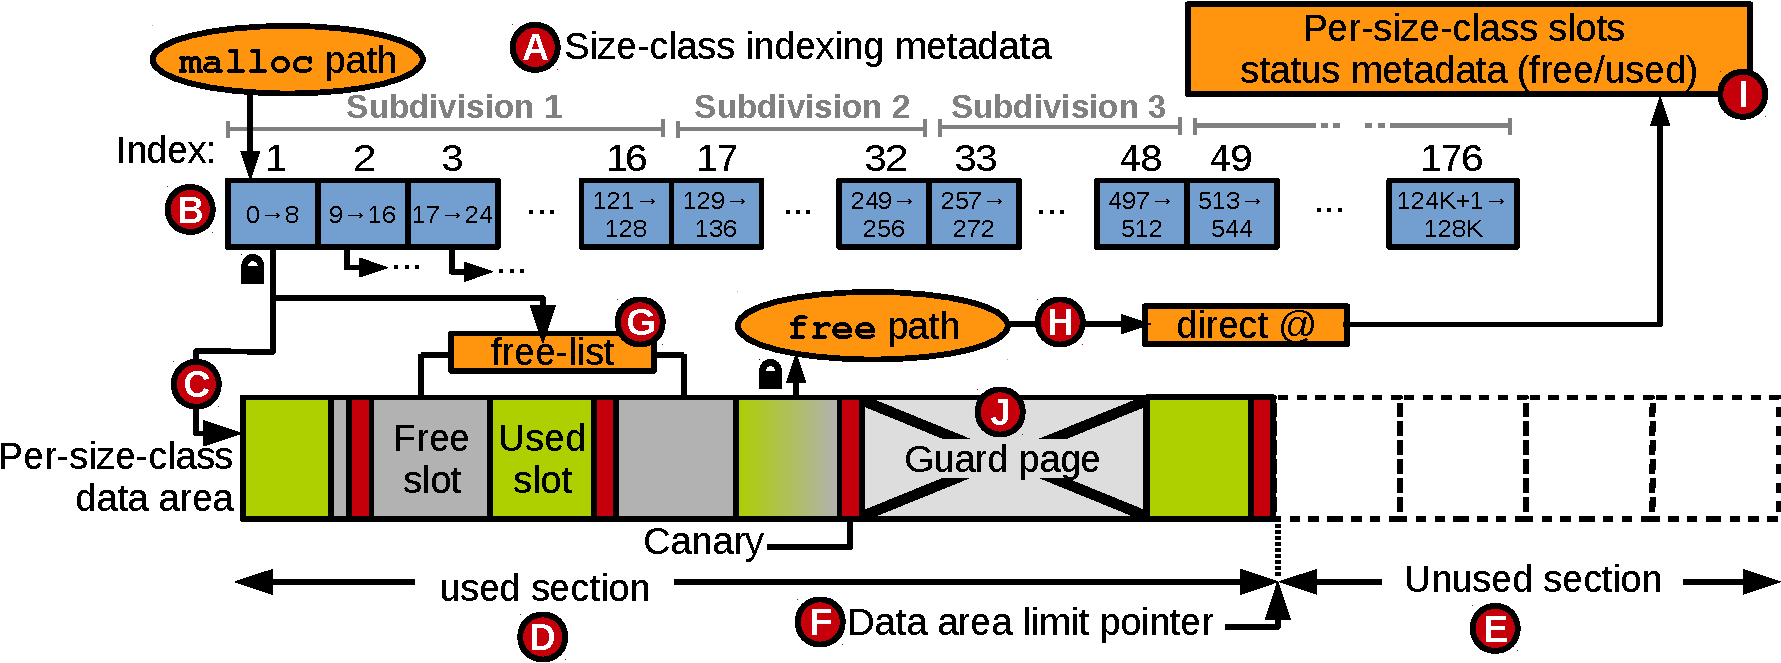
\includegraphics[scale=0.35]{overview3.pdf}
      \\ SlimGuard Design Space
    \end{figure}
\end{frame}

% Page 14
\section{Design and Implementation}
\subsection{Other Features}
\begin{frame}
		\frametitle{\secname}
    \framesubtitle{\subsecname}
    \begin{itemize}
      \item \textbf{Multithreading Support}\\
          thread-safe with fine-grained locks
      \item \textbf{Binary Compatibility}\\
          A binary Compatible dynamic library \\
            support malloc(), free(), realloc(), memalign()
    \end{itemize}
\end{frame}

% Page 15
\section{Design and Implementation}
\subsection{Security Features}
\begin{frame}
    \frametitle{\secname}
    \framesubtitle{\subsecname}
    \begin{itemize}
        \item randomization allocation
        \item metadata segradation
        \item dynamic canary
        \item guard page
        \item destroy-on-free, delayed memory reuse, etc.
    \end{itemize}
\end{frame}

% Page 16
\section{Design and Implementation}
\subsection{Randomization Allocation}
\begin{frame}
    \frametitle{\secname}
    \framesubtitle{\subsecname}
    \textbf{Goal}: make it harder to guess where the next object is located \\
    \textbf{Solution}: Build a large enough free array(G in figure)
    \begin{figure}
      \centering
      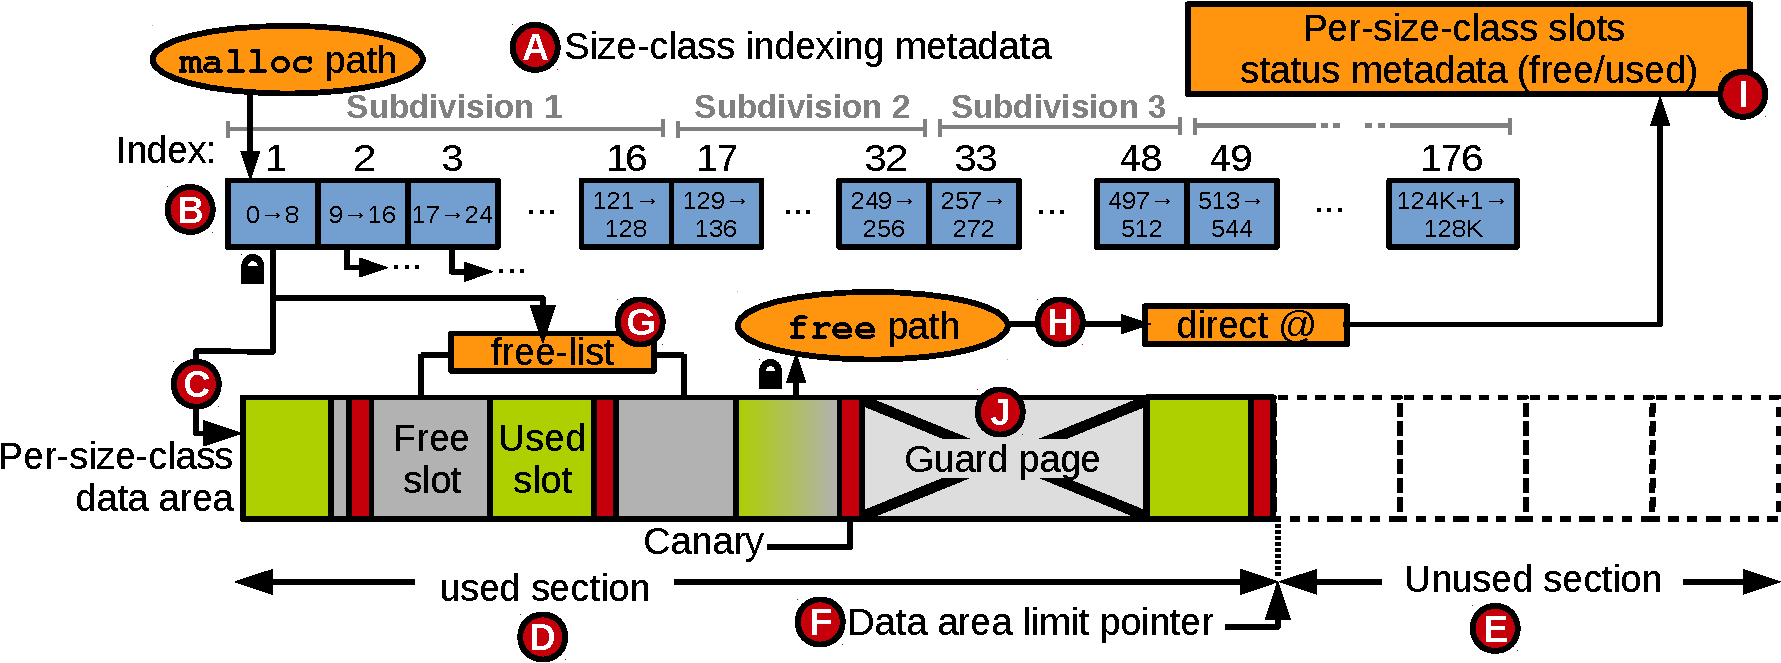
\includegraphics[scale=0.35]{overview3.pdf}
      \\ SlimGuard Design Space
    \end{figure}
\end{frame}

% Page 17
\section{Design and Implementation}
\subsection{Metadata Segregation}
\begin{frame}
    \frametitle{\secname}
    \framesubtitle{\subsecname}
    \textbf{Goal}: prevent metadata to be overwritten \\
    \textbf{Solution}: A separate region for metadata(A and B in figure)
    \begin{figure}
      \centering
      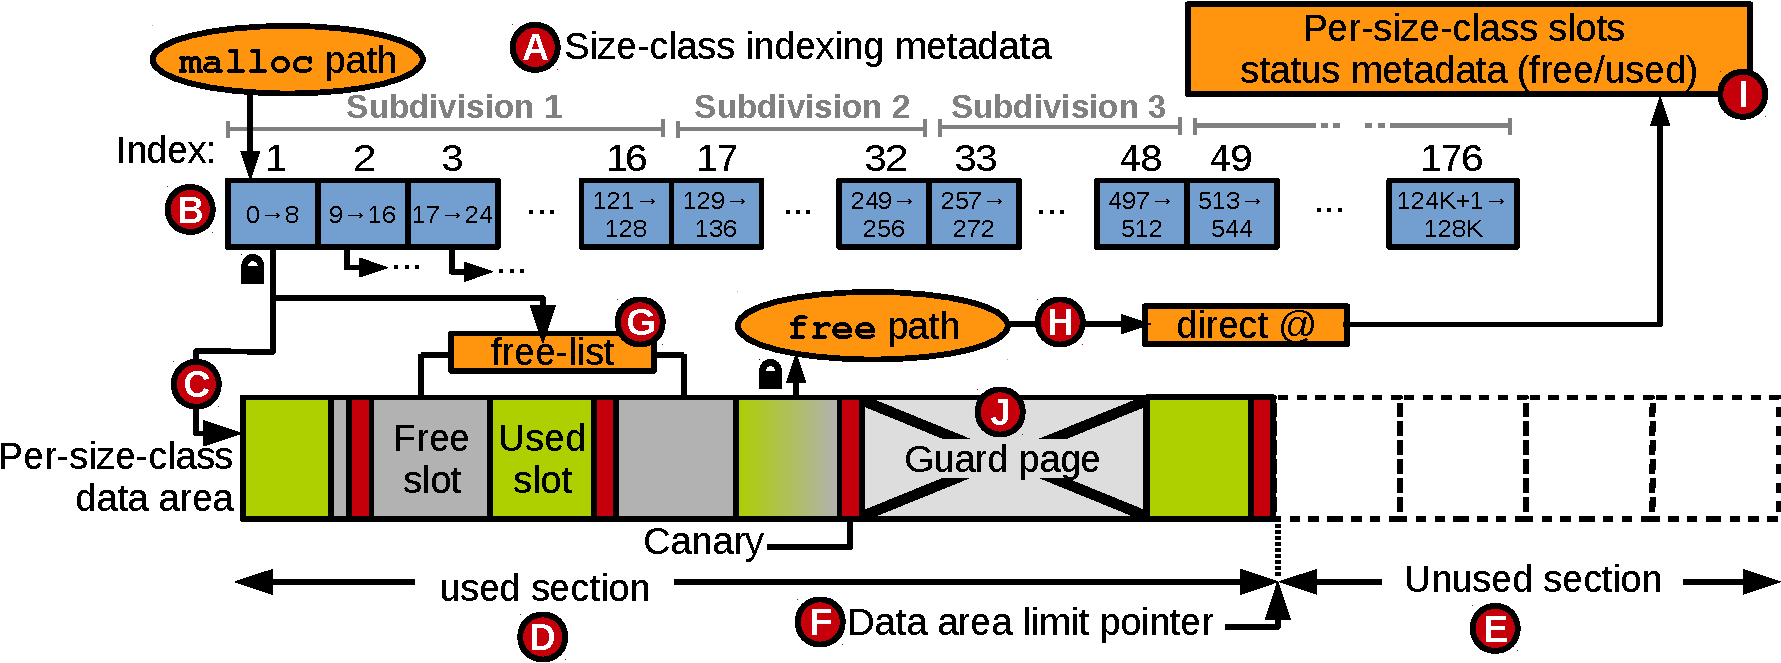
\includegraphics[scale=0.35]{overview3.pdf}
      \\ SlimGuard Design Space
    \end{figure}
\end{frame}

% Page 18
\section{Design and Implementation}
\subsection{Dynamic Canary}
\begin{frame}
    \frametitle{\secname}
    \framesubtitle{\subsecname}
    \textbf{Goal}: Detect buffer overflow \\
    \textbf{Solution}: A hashed value based on return address(red block in data area)
    \begin{figure}
      \centering
      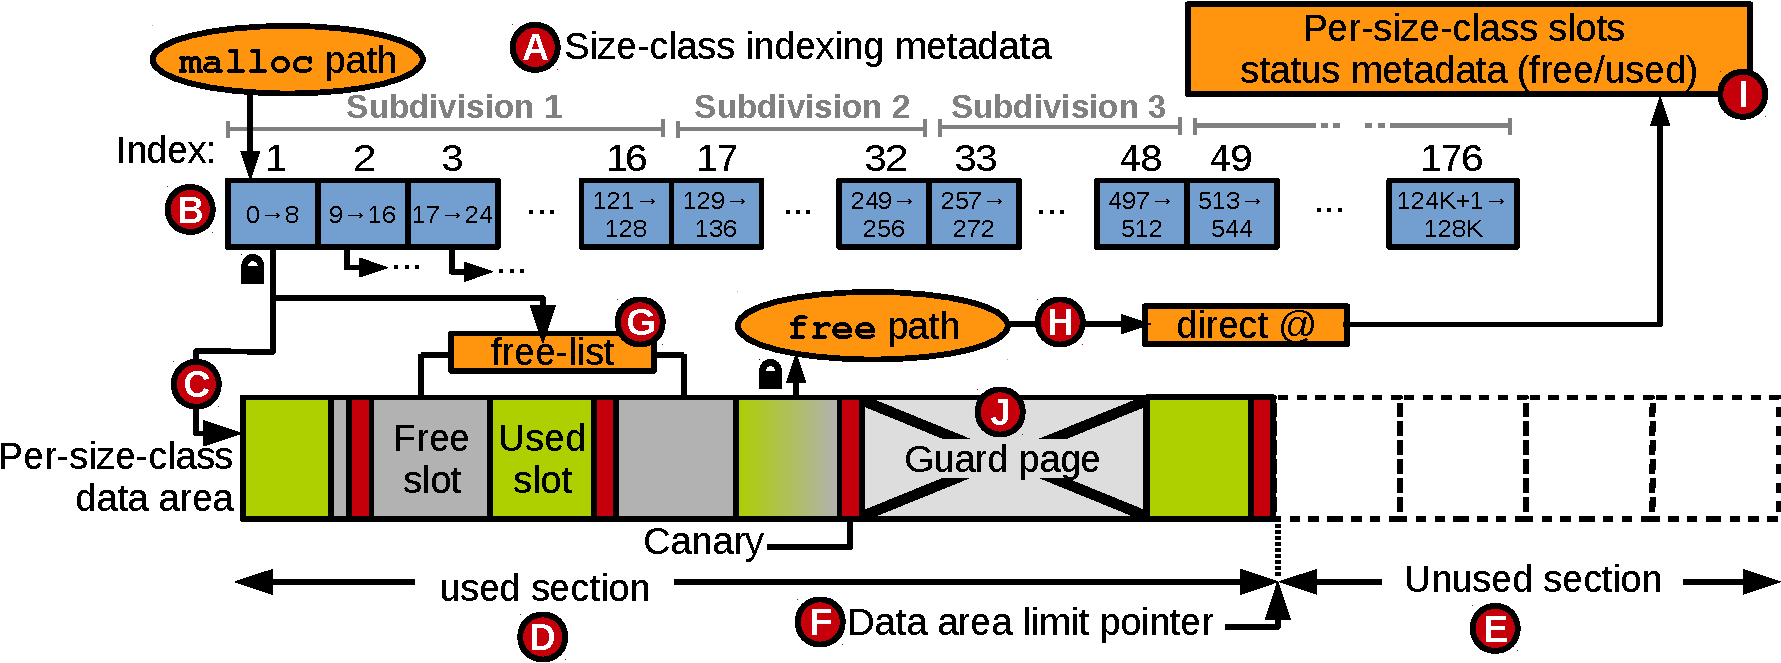
\includegraphics[scale=0.35]{overview3.pdf}
      \\ SlimGuard Design Space
    \end{figure}
\end{frame}

% Page 19
\section{Design and Implementation}
\subsection{Guard Pages}
\begin{frame}
    \frametitle{\secname}
    \framesubtitle{\subsecname}
    \textbf{Goal}: Detect buffer overflow immediately \\
    \textbf{Solution}: fully on demand guard pages(J in figure)
    \begin{figure}
      \centering
      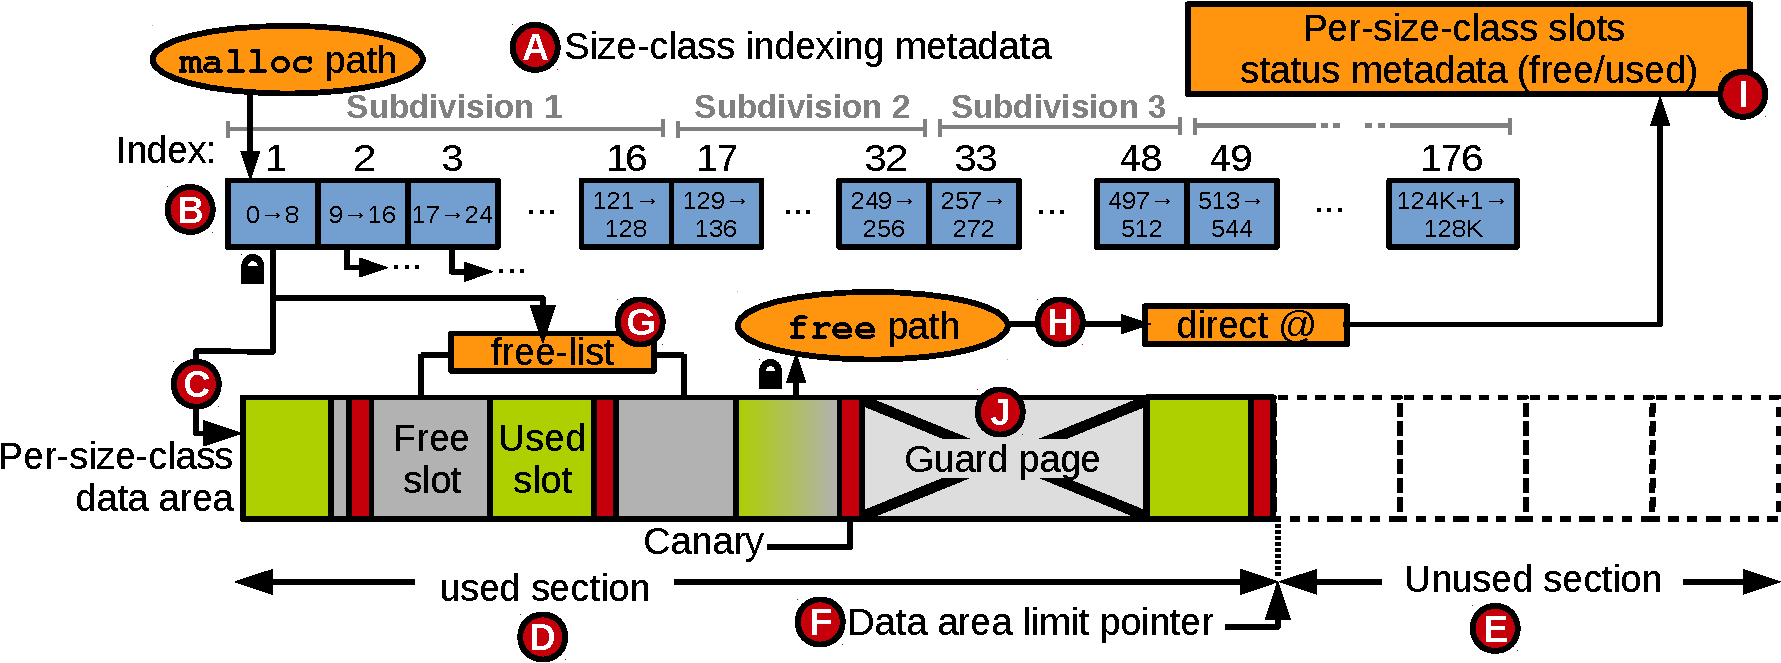
\includegraphics[scale=0.35]{overview3.pdf}
      \\ SlimGuard Design Space
    \end{figure}
\end{frame}


% Page 20
\section{Design and Implementation}
\subsection{Other Security Features}
\begin{frame}
    \frametitle{\secname}
    \framesubtitle{\subsecname}
    \begin{itemize}
        \item Destroy-on-Free\\
            zero out the free area
        \item delayed memory reuse\\
            a side-effect from our randomization
    \end{itemize}
\end{frame}

% Page 21
\section{Results}
\subsection{Performance and Memory Overhead Analysis}
\begin{frame}
		\frametitle{\secname}
    \framesubtitle{\subsecname}
    \begin{figure}
      \centering
      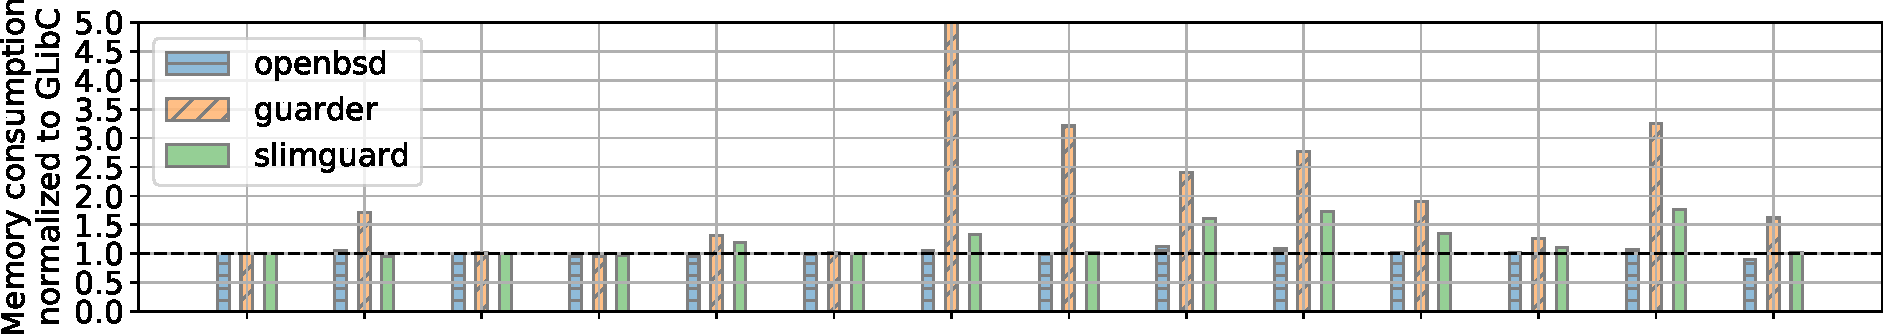
\includegraphics[scale=0.3]{macro-mem.pdf}
      \\
      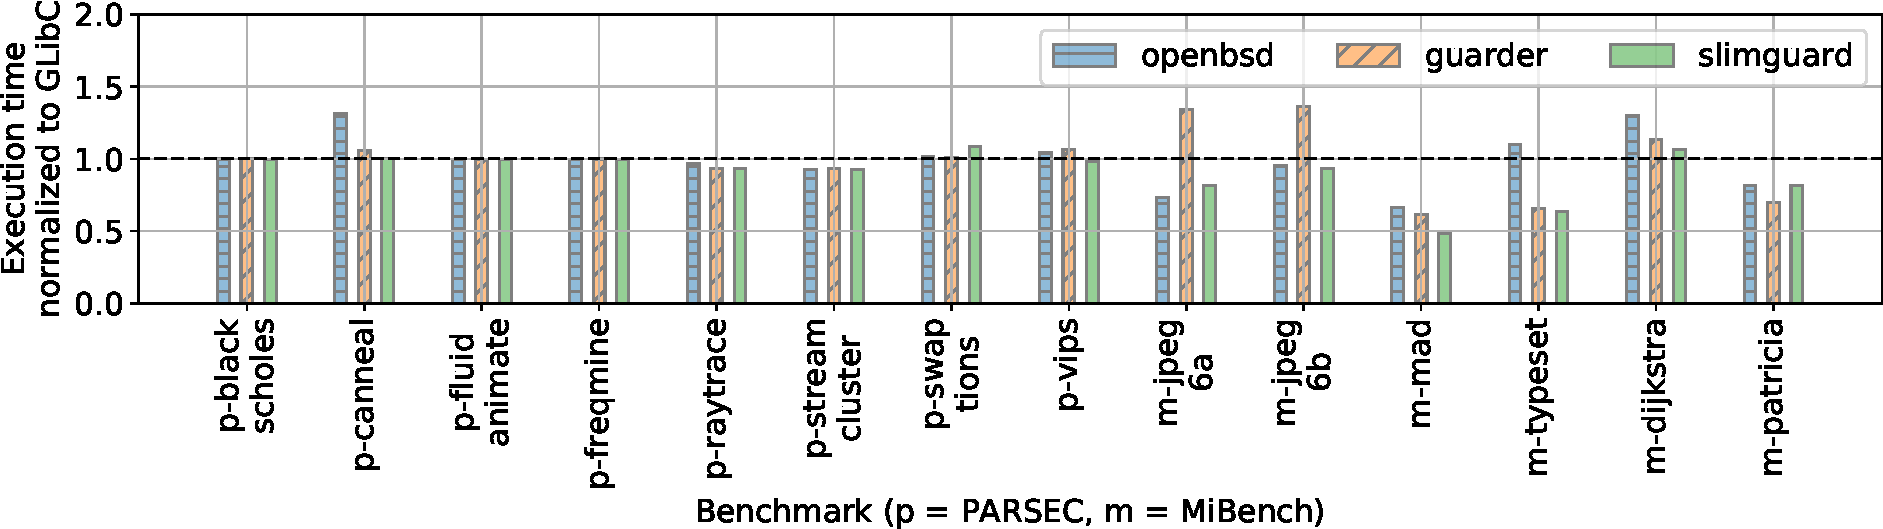
\includegraphics[scale=0.3]{macro-time.pdf}
      \\Memory footprint (top) and execution time (bottom) of SlimGuard,
      OpenBSD and Guarder for PARSEC (\texttt{p-*}) and MiBench (\texttt{m-*})
      macro-benchmarks. All values are normalized to Glibc's memory footprint
      and execution time.
    \end{figure}
\end{frame}

% Page 22
\section{Results}
\subsection{Multitheading}
\begin{frame}
		\frametitle{\secname}
    \framesubtitle{\subsecname}
    \begin{figure}
      \centering
      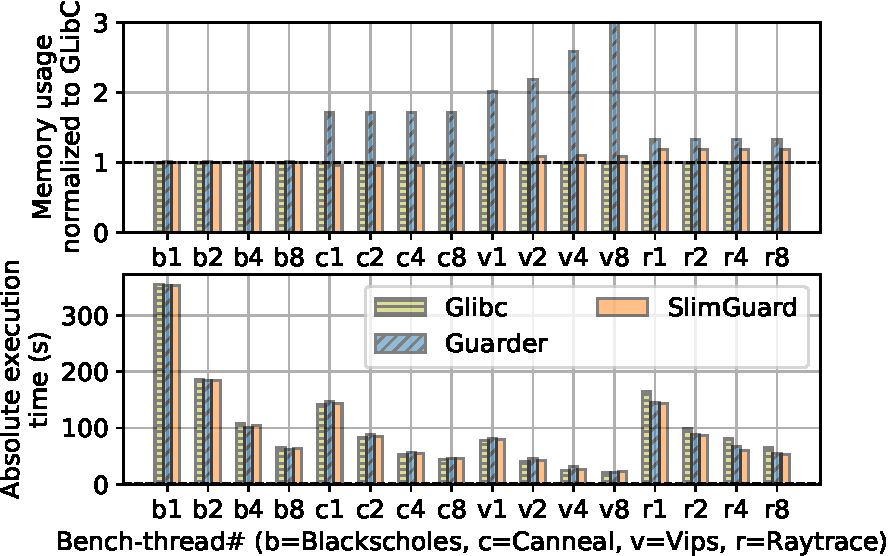
\includegraphics[scale=0.6]{multithreading.pdf}
      \\Multithreading memory overhead (top) and performance (bottom)
      results.

    \end{figure}
\end{frame}

% Page 23
\section{Results}
\subsection{Security Analysis}
\begin{frame}
    \frametitle{\secname}
    \framesubtitle{\subsecname}
    SlimGuard's efficiency on real-world bugs
    \begin{columns}
       \begin{column}{0.5\textwidth}
            \begin{itemize}
                \item gzip-1.2.4
                \item ncompress-4.2.4
                \item ed-1.14.1
                \item ImageMagic 7.0.4-1
            \end{itemize}
       \end{column}

       \begin{column}{0.5\textwidth}
           \textbf{SlimGuard successfully detects the exploit in all cases.}

       \end{column}
    \end{columns}

\end{frame}


% Page 24
\section{Conclusion}
\begin{frame}
	\frametitle{\secname}

            \begin{itemize}
                \item Memory overhead is not acceptable in the state-of-the-art memory allocator
                \item Slimguard: memory-efficient and secure allocator
                \item Memory overhead is much smaller than state-of-the-art allocator
            \end{itemize}
\end{frame}

% Page 25
\section{SlimGuard's Source Code}
\begin{frame}

    \frametitle{\secname}
    SlimGuard\footnotemark is an open-source project of the Systems Software Research Group
    at Virginia Tech.
\\
    Source Available at \textbf{https://ssrg-vt.github.io/SlimGuard/}
\\
    Docker with benchmarks available at \\
    \textbf{https://hub.docker.com/repository/docker/bcliu430/slimguard}

    \footnotetext{SlimGuard is supported in part by ONR under grants N00014-16-1-2104 and
    N00014-18-1-2022.
    \\
    }
\end{frame}

\end{document}
